\section{Achieve Shuffle Optimization}
In this section, we try to achieve shuffle optimization by applying
\begin{itemize}
	\item Decoupling shuffle from task
	\item Pre-fetching shuffle to reduce node
\end{itemize}
on the DAG computing framwork.
We choose Spark as the representative of DAG computing framwork to implement our optimizations.
\subsection{Decouple shuffle from task}
On the map task side of shuffle, it's used to partition the output of map task according to the pre-defined partitioner. More specifically, shuffle takes a set of key-value pairs as input. And then it calculates the partitioner number of a key-value pair by applying pre-defined the partition function to the key. At last it put the key-value pair into the corresponding partition. The output at last is a set of blocks,each of them containing the key-value pairs for one partition. For those application context unrelated blocks, they can be easily hijacked in the memory of Spark executor and moved out of JVM space via memory mapping. Meanwhile, we have to prevent the memory spill(memory leak?) during the shuffle partition procedure, so that the shuffle data can never reach the disk. The default shuffle spill threshold in Spark is 5GB\cite{sparksource}, which is big enough in most scenarios according to Section \ref{shufflesize}.

\subsection{Pre-schedule with Application Context}
When the shuffle output blocks are available in memory, they can be pre-fetched to remote hosts to hide the network transfer time(latency). But at that time, the reduce tasks taking shuffle as input (consuming shuffle output?)are still pending. In other word, the remote hosts of those blocks keep unknown until the reduce tasks are scheduled by the DAG framework. In order to break this serialization between map tasks and shuffle, we have to first pre-schedule the task-node mapping ahead of DAG framework scheduler. We explore several pre-scheduling schemes in different scenarios, and evaluate the performance of pre-scheduling and prediction by calculating the improvement of reduce tasks completion time with trace of OpenCloud\cite{opencloudtrace}. We first emulate the scheduling algorithm of Spark to schedule the reduce tasks of one job, and take the bottleneck of the task set as the completion time. Then we remove the shuffle read time as the assumption of shuffle data pre-fetch and emulate under different schemes. The result is shown in \ref{fig:sim}.
\begin{figure*}
	\centering
	\begin{minipage}{0.34\linewidth}
		\begin{figure}[H]
			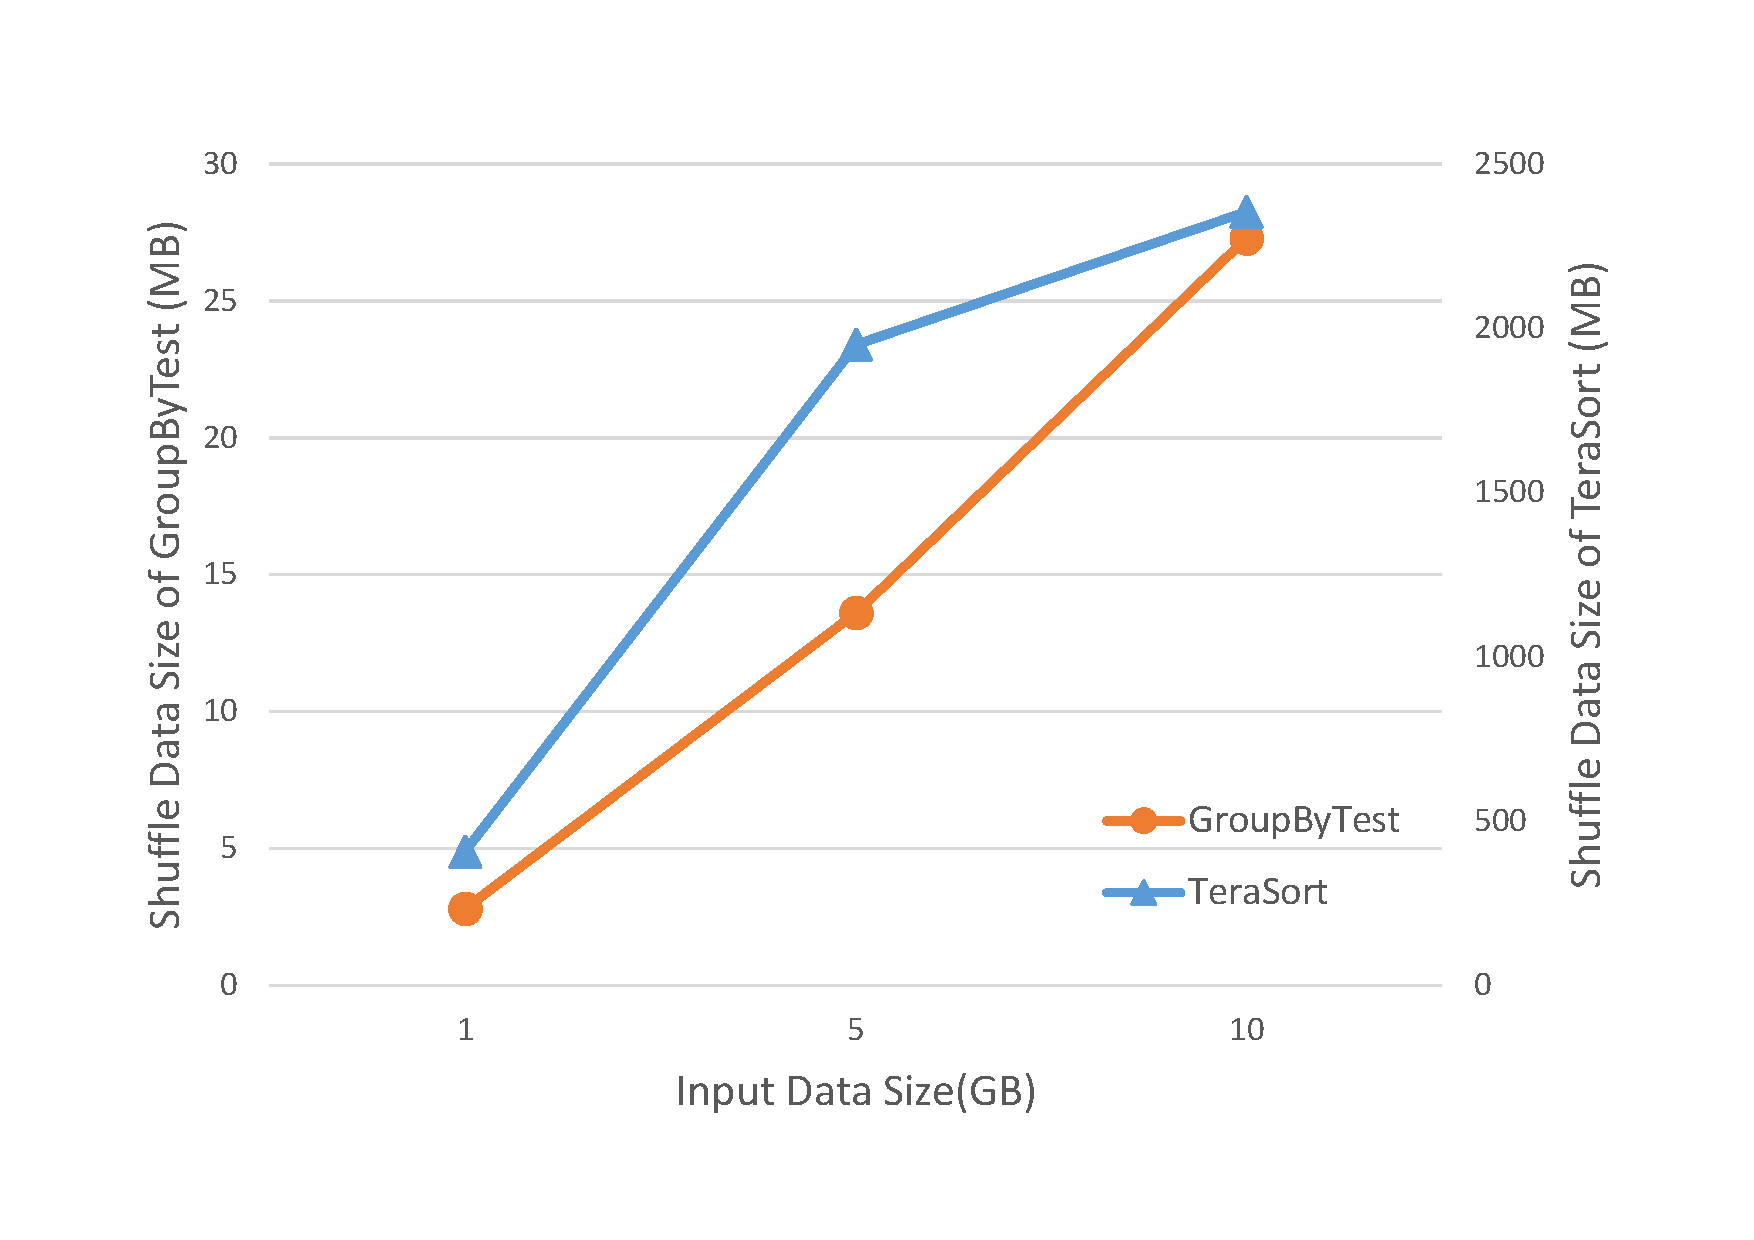
\includegraphics[width=\textwidth]{fig/shuffle_size}
			\caption{Shuffle Size Comparing with Input Size}
			\label{fig:shuffle_size}
		\end{figure}
	\end{minipage}
	\begin{minipage}{0.65\linewidth}
		\begin{figure}[H]
			\begin{subfigure}{0.5\textwidth}
				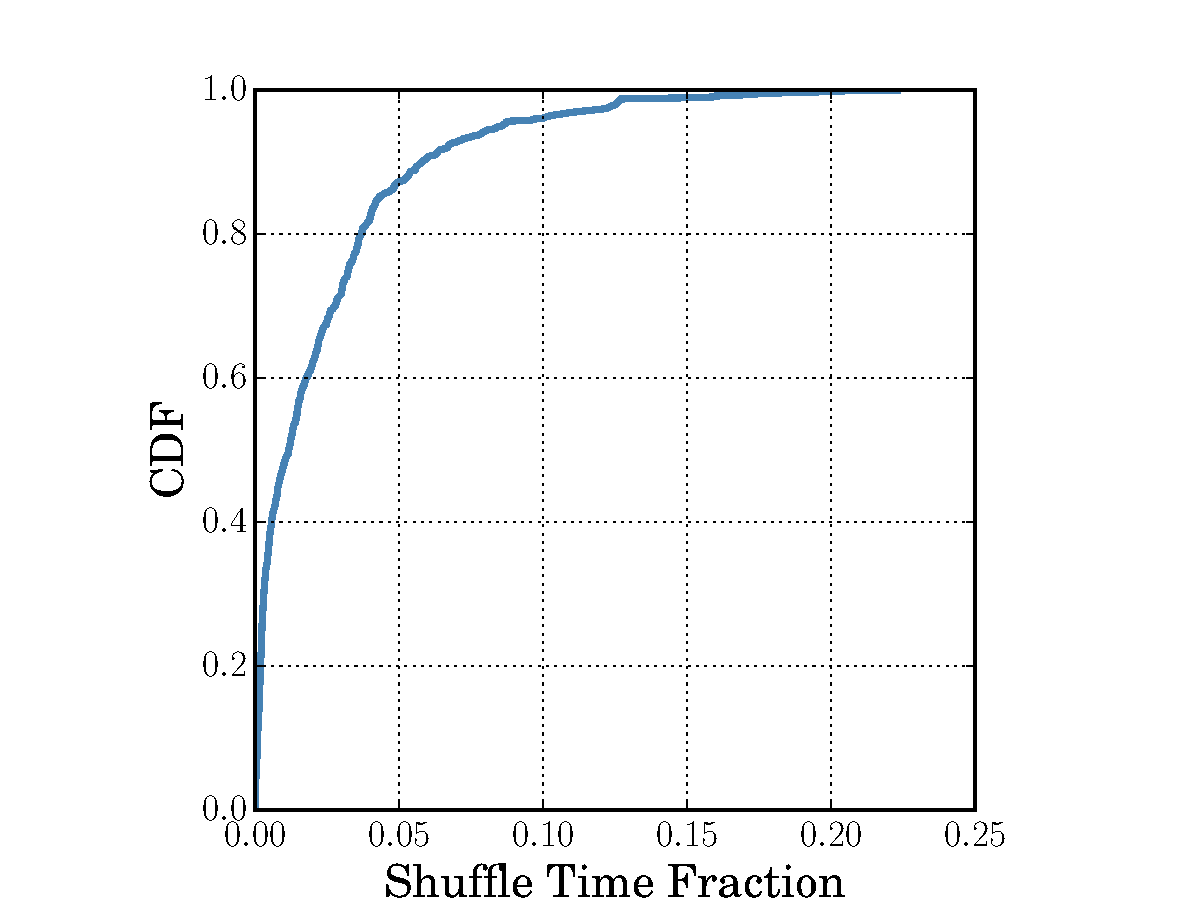
\includegraphics[width=\linewidth]{fig/reduce_cdf}
				\caption{Shuffle Time Fraction CDF}
				\label{fig:cdf}
			\end{subfigure}	
			\begin{subfigure}{0.5\textwidth}
				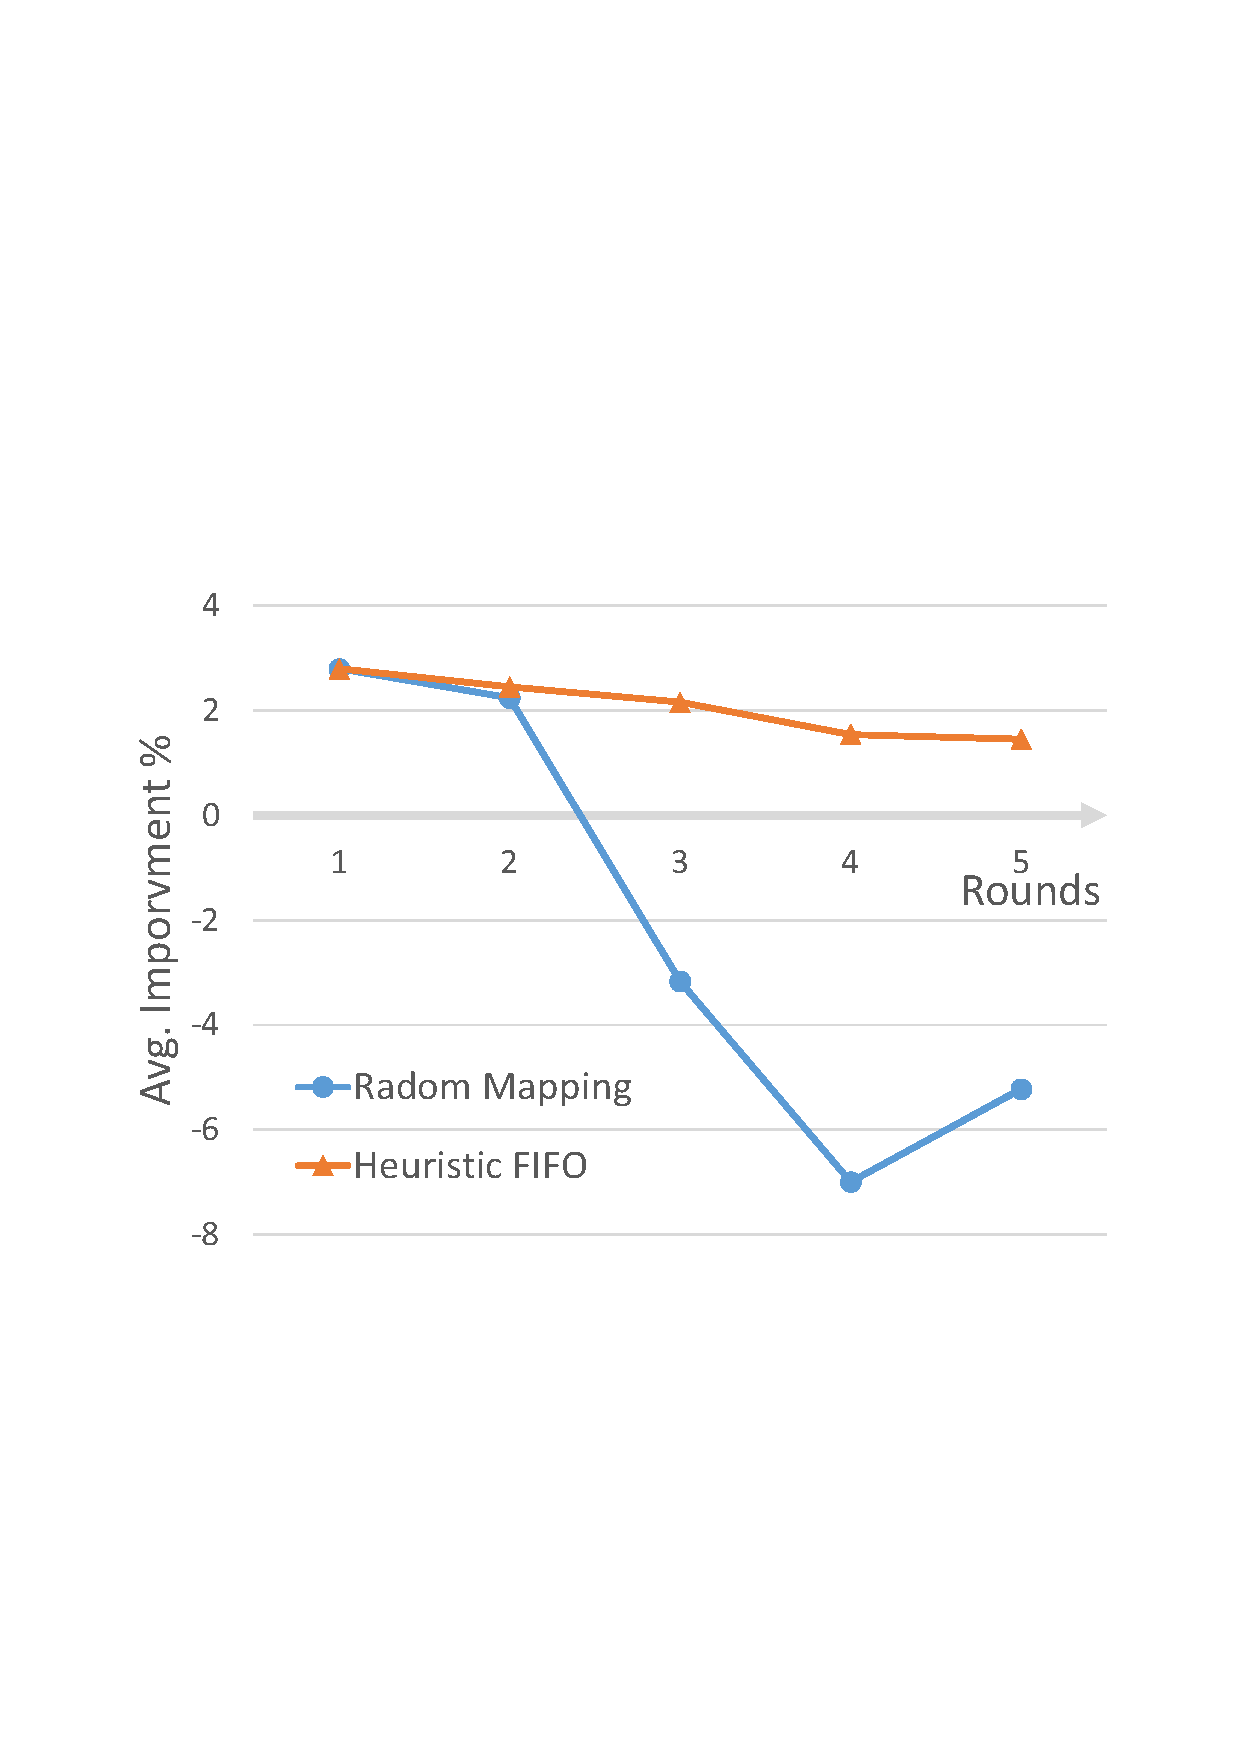
\includegraphics[width=\linewidth]{fig/sim}
				\caption{Stage Completion Time Improvement}
				\label{fig:sim}
			\end{subfigure}	
			\caption{Emulate Result of OpenCloud Trace}
		\end{figure}
	\end{minipage}
\end{figure*}
Note that since most of the traces from OpenCloud is shuffle-light workload as shown in Figure \ref{fig:cdf}. The average shuffle read time is 2.3\% of total reduce completion time. So we will only use this trace to evaluate the pre-scheduling. 
\subsubsection{Random Task-Node Mapping}\label{randomassign}
The simplest way of pre-scheduling is mapping tasks to different nodes evenly. As shown in Figure \ref{fig:sim}, Random mapping works well when there is only one round of tasks in cluster. But multi-round in cluster is overwhelming according to Section \ref{multi}. The performance of random mapping collapses as the round number grows. After analyzing the trace, we find out that it's caused by data-skew. Reports in these papers\cite{skewtune, reining, gufler2012load} also claim that data-skew is common in data-parallel computing. When we apply a random mapping, it's probable to assign several slow tasks on one node. The collision then slow down the whole stage, which makes the performance even worse than those without shuffle-prefetch. In addition, randomly-assigned tasks also ignore(fail to consider) the data locality (problem) between shuffle map output and shuffle reduce input, which can bring extra network traffic in cluster. 


\subsubsection{Shuffle Output Prediction}\label{shuffleprediction}
The failure of random mapping was obviously caused by application context (e.g. Shuffle input of each task) unawareness(the unawareness of application context), which results in a severe data skew. To avoid the 'bad' schedule results, we have to leverage the application context as assistance. The optimal schedule decision can be made under the awareness of shuffle dependencies number with input size for each task. Unfortunately these data is unavailable when the shuffle-prefetch starts. But the approximate size of each reduce task can be predicted during the initial phase of map tasks with DAG context, so that the scheduling can approach a more uniform load for each node.

According to the DAG computing process, the shuffle size of each reduce task is decided by the input data, map task computation and the hash partitioner. And for each map task, it will produce a data block for each reduce tasks, like '1-1' in Figure \ref{fig:shuffle}. '1-1' means it's produced by 'Map Task 1' for 'Reduce Task 1'. For Hadoop MapReduce, the shuffle input for each reduce task can be predicted with decent accuracy\cite{ishuffle}. They propose a liner regression model based on Verma et al.\cite{predict} that the ratio of map output size and input size is invariant given the same job configuration. Several map outputs (marked as Map Output in Figure \ref{fig:shuffle}) are picked as observation objects to train the model and then predict the final reduce distribution. But in the more sophisticated DAG computing framework like Spark, this model doesn't fit. For instance, the reduce stage in Spark has more tasks that consume shuffle data instead of Hadoop MapReduce.(than Hadoop MapReduce?) More importantly, the customized partitioner can bring(introduce) huge inconsistency between observed map output blocks distribution and the final reduce distribution, as we presented in Figure \ref{fig:dis}. We use different datasets with different partitioners to find the connection among these three factors. We normalize threes sets of data to [0,1] to fit in one figure. In Figure \ref{fig:hash_pre}, we use a random input dataset with the Hash Partitioner of Spark\cite{sparksource}. In Figure \ref{fig:range_pre_sample}, we use a skew dataset with the Range Partitioner of Spark\cite{sparksource}.
We randomly pick one observation map output and plot. As we can see, in hash partitioner, the distribution of each map(blue area) is close to the final reduce distribution(orange boxes). The prediction results also turns out well fitted. As we apply linear regression model to predict the final reduce distribution of Range Partitioner. The prediction is severely effected(affected) by the skew observed map output distribution. 

To avoid this inconsistency in some cases, we introduce another methodology, weighted reservoir sampling, to mitigate this inconsistency. The classic reservoir sampling is designed for randomly choosing(choosen) \textit{k} samples from \textit{n} items, where \textit{n} is either a very large or an unknown number\cite{reservoir}. For each partition of data that produces shuffle output, we use reservoir sampling to randomly pick $s \times p$ of samples, where $p$ is the number of reduce tasks and $s$ is a tunable number. The number of input data partition and reduce tasks can be easily obtained when the (??)from the DAG information. In Figure \ref{fig:range_pre_sample}, we set $s = 3$. After that, the map function is called locally to process the sampled data. As the 'Sampling' part shown in Figure \ref{fig:shuffle}, the final sampling map outputs are collected with the size of each partition of input data which is used as weight for each set of sample. For each reduce, the predicted size $reduceSize_i$

\begin{equation}
\label{equationsample} 
\begin{aligned}
	reduceSize_i = {\displaystyle\sum_{j=0}^{m} {partitionSize_j \times \frac{sample_i}{s \times p}}} \\ 
	{\left( m = \text{partition number of input data} \right)}
\end{aligned}
\end{equation}
As we can see in Figure \ref{fig:range_pre_sample}, the prediction result is much better even in a very skew scenario. The variance of the normalized data of sampling prediction is because the standard deviation of the prediction result is relatively small comparing(compared) to the average prediction size, which is $0.0015$ in this example. Figure \ref{fig:prediction_relative_error} further proves that the sampling prediction can provide precise results even in the absolute partition size of reduce tasks. On the opposite, the result of linear regression comes out with huge relative error comparing(compared) with the fact of partition size of reduce tasks.
\begin{minipage}{\linewidth}
\begin{algorithm}[H]
\caption{Heuristic MinHeap Scheduling for Single Shuffle}
\label{hminheap}
	\begin{algorithmic}[1]
	\small
	\Procedure{schedule}{$m, h, p\_reduces$}
		\State $R\gets$ sort $p\_reduces$ by size
		\State $M\gets$ mapping of host id in $h$ to reduce id and size
		\State $rid\gets$ len$\left(R\right)$
		\Comment{Current scheduled reduce id}
		\While{$rid \geq 0$}
		\Comment{Schedule redues by MinHeap}
		\State Update $M\left[0\right].size$
		\State Assign $R\left(rid\right)$ to $M\left[0\right]$
		\State sift\_down$\left(M\left[0\right]\right)$
		\State
		\Comment{Use min-heap according to size in $M$}
		\State $rid\gets rid-1$
		\EndWhile
		\State $max\gets$ maximum size in $M$
		\State $rid\gets$ len$\left(R\right)$
		\While{$rid \geq 0$}
		\Comment{Heuristic swap by locality}
		\State $prob\gets$ max composition portion of $rid$
		\State $nor\gets \left(prob-1/m\right)/\left(1-1/m\right)/10$
		\State
		\Comment{Use $nor$ to limit the performance degradation in tasks swap}
		\State $t\_h\gets$ host that produces $prob$ data of $rid$
		\State $c\_h\gets$ current assigned host by MinHeap
		\If{$t\_h == c\_h$}
			\State Seal the assignment of $rid$ in $M$
		\Else
			\State swap\_tasks$\left(rid, c\_h, t\_h, max, nor\right)$
		\EndIf
		\State $rid\gets rid-1$
		\EndWhile
		% \Comment{$m$ is the number of input data}
		% \Comment{$r$ is partition number of reduces}
		% \Comment{$hosts$ is array of (hostid, partitionids[], size)}
		% \Comment{$c$ is $r*m$ array of composition data}
		% \Comment{$pSize$ is $r$ size array of predicted size of reduces}
		\Return $M$
	\EndProcedure
	\Procedure{swap\_tasks}{$rid, c\_h, t\_h, max, nor$}
	\State $num\gets$ number of reduces 
	\State selected from $t\_h$ that $total\_size$ won't
	\State make both $c\_h$ and $t\_h$ exceed $\left(1+nor\right)*max$
	\State after swapping
	\If{$num == 0$}
		\State return
	\Else
		\State \# Swap $nums$ of reduces with $rid$ between $c\_h$ and $t\_h$
		\State \# Update size of $t\_h$ and $c\_h$
	\EndIf
	\EndProcedure
	\end{algorithmic}
\end{algorithm}
\end{minipage}

But the sampling prediction may introduce a extra overhead in DAG computing process, we will evaluate the overhead in the Section \ref{evaluation}. Though in most cases, the overhead is negligible, but we won't use sampling for every reduce prediction. Combing with the DAG context, the sampling prediction will be triggered only when the range partitioner or customized partitioner occurs.

\subsubsection{Heuristic MinHeap Scheduling of Single Shuffle}\label{h-minheap}
For each predicted reduce size, a percentage array of total data composition among each map output is calculated. The highest percentage and it's corresponding host should be the best choice the dimension of locality. In order to achieve the uniform load on each node while reducing the network traffic and shuffle transmission time. With this composition array and the predicted size of reduce, we present a heuristic MinHeap as the scheduling algorithm for single shuffle.

This algorithm can be divided into two round of scheduling. For input of $schedule$, $m$ is the partition number of input data, $h$ is the array of nodes ID in cluster and $p\_reduces$ is the predicted reduce matrix. Each row in $p\_reduces$ contains $r\_id$ as reduce partition ID, $size$ as predicted size of this partition, $prob$ as the maximum composition portion of reduce data, and $host$ as the node ID that produce the maximum portion of reduce data. As for $M$, it's a matrix consists $hostid$, $size$(total size of reduce data on this node) and an array of reduce id. 

In the first round (i.e. The first while in Algorithm \ref{hminheap}), the reduces are first sorted by size. And then, they are assigned to hosts in the descending order of size . For hosts, we use a min-heap to maintain the hosts array according to the scheduled size on each hosts. In other word, the heavy tasks can be distributed evenly in the cluster.  After the scheduling, the completion time of reduce stage is close to the optimal. \textcolor{red}{may need to add math prove between this and optimal}. In the second round, the task-host mapping will be adjusted according to the locality. The closer $prob$ is to $1/m$, the more evenly this reduce is distributed in cluster. For a task which contains at most $prob$ data from $host$, the normalized probability $nor$ is calculated as a bound of performance degradation. This normalization can ensure that the more performance can be traded when the locality level increases. But the degradation of performance will not exceed 10\% since the maximum value of nor is 0.1 (in extreme skew scenarios).  If the assigned host($c\_h$ in algorithm \ref{hminheap}) is not equal to the $host$ ($t\_h$ in algorithm \ref{hminheap}), than it has the $nor$ probability to trigger a tasks swap between two hosts. To maintain the scheduling mapping of first round, the tasks will only be swapped if the target hosts owns a set of tasks that has similar size totally. We use the OpenCloud\cite{opencloudtrace} trace to evaluate Heuristic MinHeap. Without swapping, the Heuristic MinHeap can achieve a better performance improvement (average 5.7\%) than the default Spark FIFO scheduling algorithm (average 2.7\%). In the case of extreme skew scenario, such as Figure \ref{fig:range_pre_sample}, Heuristic MinHeap trades about 0.05\% percent of stage completion time for 99\% reduction of shuffle data transmission through network by heuristicly swapping tasks.

\begin{figure}
	\centering
	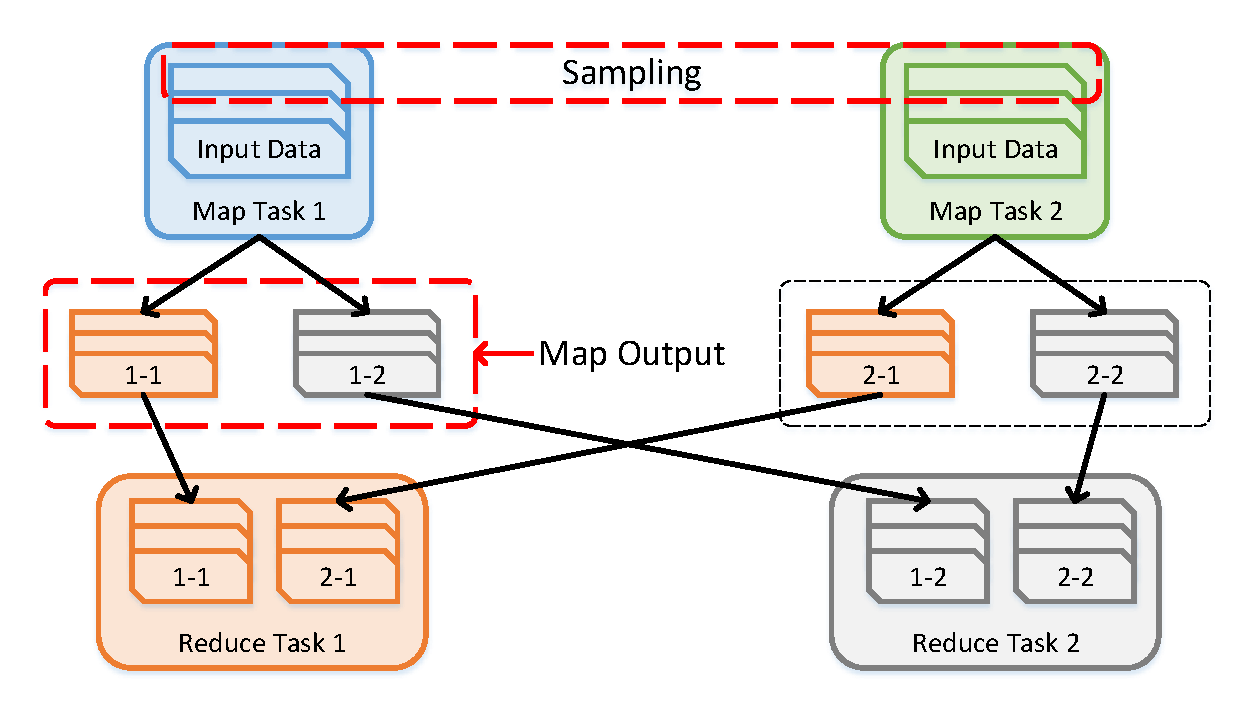
\includegraphics[width=\linewidth]{fig/shuffle}
	\caption{Shuffle Data Prediction}
	\label{fig:shuffle}
\end{figure}

\begin{figure*}
	\centering
	\begin{subfigure}[b]{0.32\linewidth}
		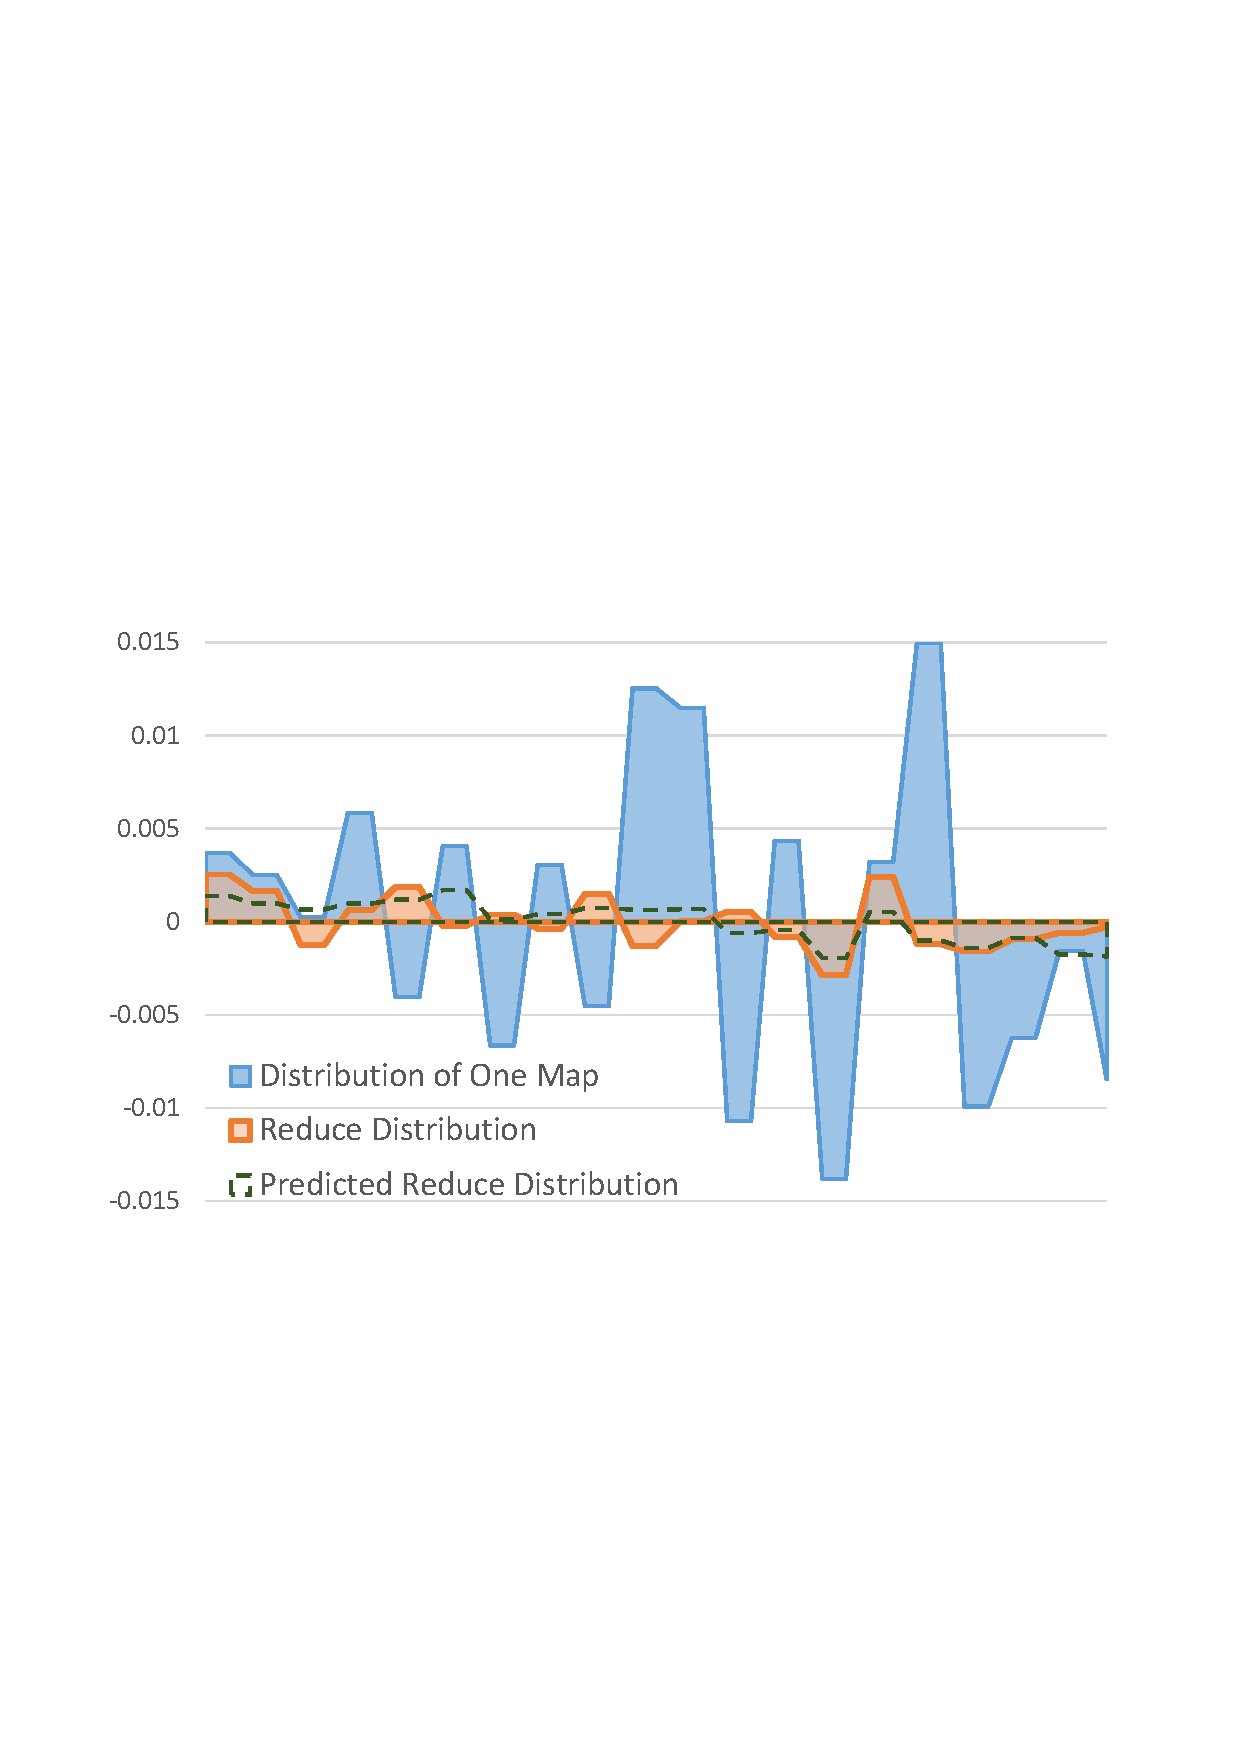
\includegraphics[width=\linewidth]{fig/hash_pre}
		\caption{Linear Regression Prediction of Hash Partitioner}
		\label{fig:hash_pre}
	\end{subfigure}
	\begin{subfigure}[b]{0.32\linewidth}
		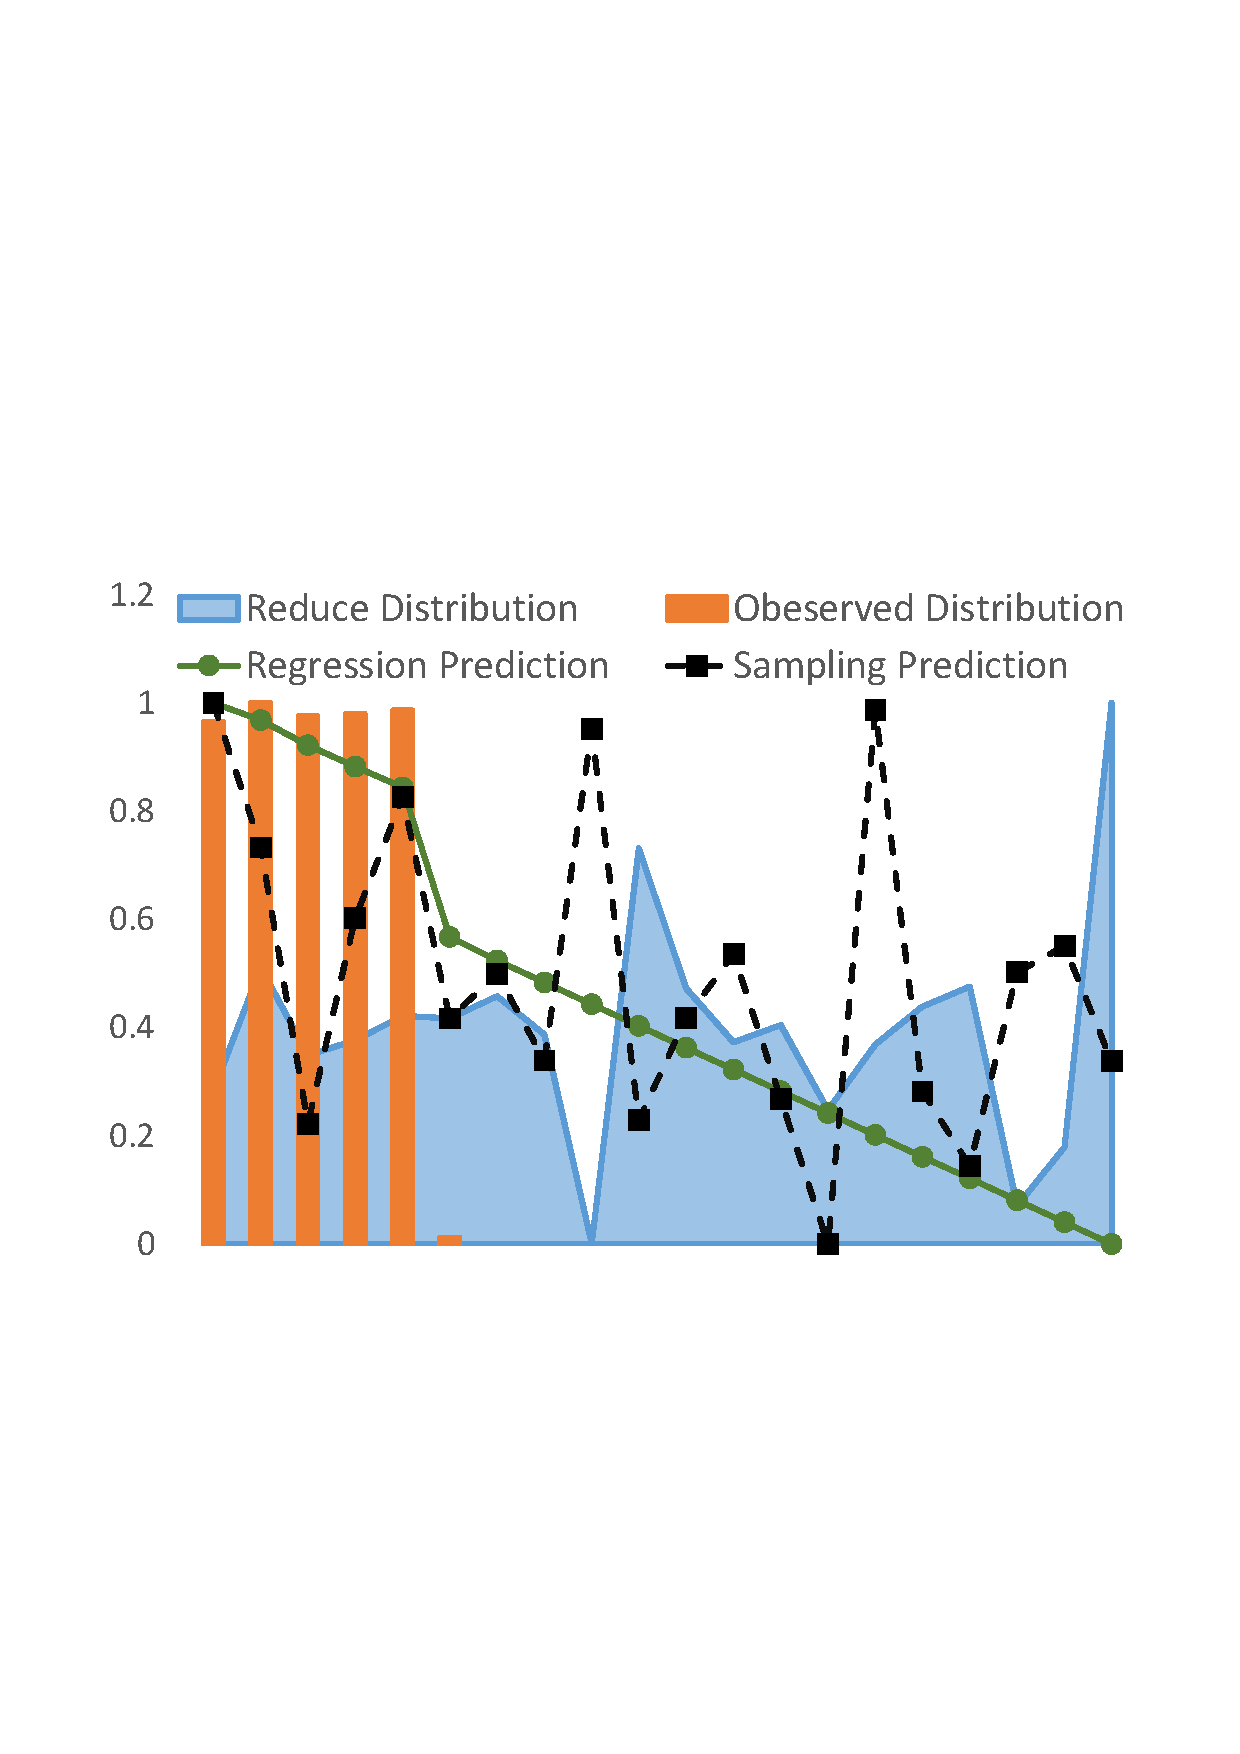
\includegraphics[width=\linewidth]{fig/range_pre_sample}
		\caption{Linear Regression and Sampling Prediction of Range Partitioner}
		\label{fig:range_pre_sample}
	\end{subfigure}
	\begin{subfigure}[b]{0.32\linewidth}
		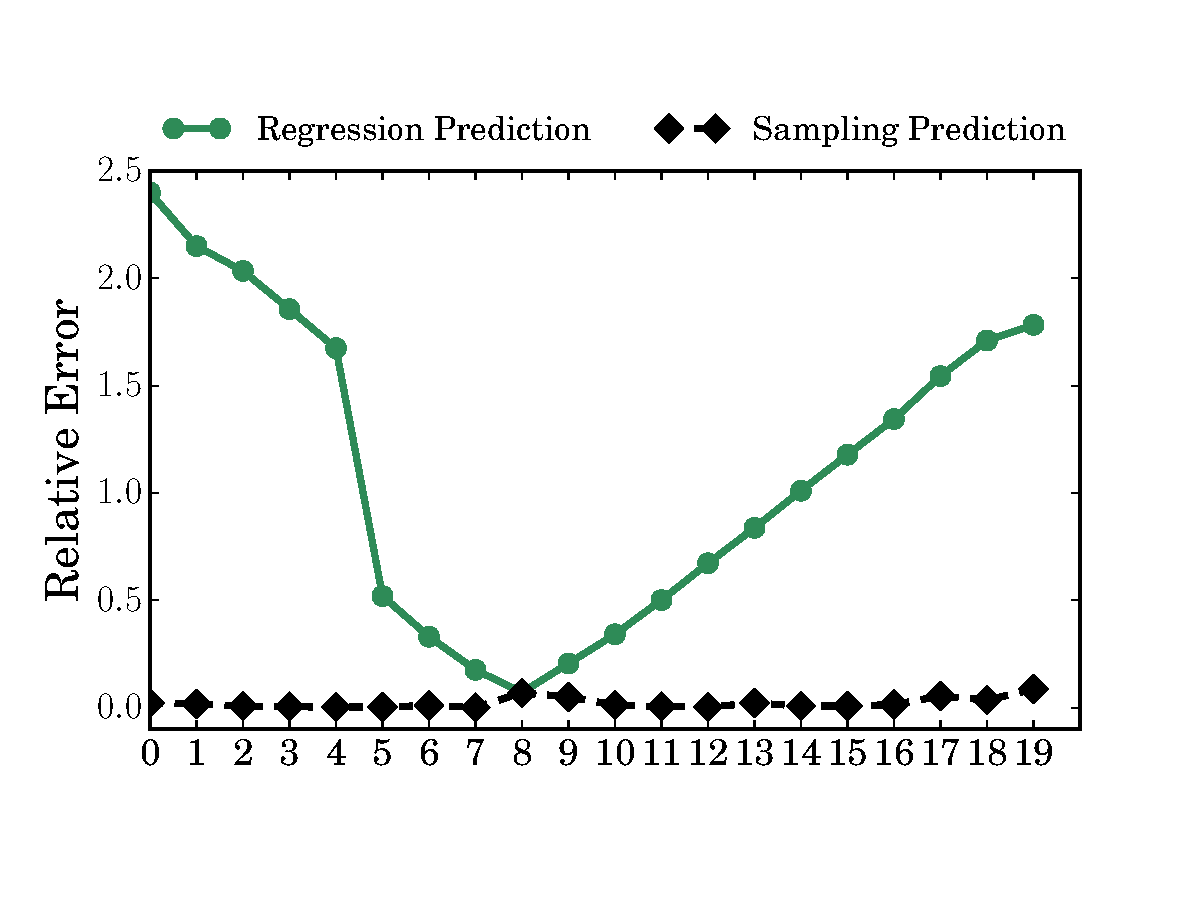
\includegraphics[width=\linewidth]{fig/prediction_relative_error}
		\caption{Prediction Relative Error of Range Partitioner}
		\label{fig:prediction_relative_error}
	\end{subfigure}
	\caption{Reduction Distribution Prediction}
	\label{fig:dis}
\end{figure*}
\subsubsection{Cope with Multiple Shuffles}
Unlike Hadoop MapReduce, multiple shuffles commonly exist in DAG computing. The techniques mention in Section \ref{shuffleprediction} can only predict the ongoing shuffle. For those pending shuffle, it's impossible to predict their size because of lacking either observed map outputs or sampling data. Let all tasks of all shuffle to be scheduled by DAG framework simultaneously can relieve the dilemma. But huge modification in DAG framework should be made by doing this. For example, Spark only supports one stage running at the same time for one application. To avoid this redundant workload, we provide the accumulating scheduling to cope with multiple shuffles.
\begin{minipage}{\linewidth}
\begin{algorithm}[H]
\caption{Accumulate Scheduling for Multi-Shuffles}
\label{mhminheap}
	\begin{algorithmic}[1]
	\small
	\Procedure{mSchedule}{$m, h, p\_reduces, shuffles$}
		\State
		\Comment $shuffles$ is the previous array of reduce partition ID, host ID and size
		\ForAll{$r\_id$ in $p\_reduces$}
		\State $p\_reduce\left[r\_id\right].size\gets p\_reduce\left[r\_id\right].size + shuffles\left[r\_id\right].size$
		\If{$shuffles\left[r\_id\right].size\geq p\_reduce\left[r\_id\right].size * p\_reduce\left[r\_id\right].prob$}
		\State Update $prob$ set $host$ to $shuffles\left[r\_id\right].host$
		\EndIf
		\EndFor
		\State $M\gets$ schedule$\left(m, h, p\_reduecs\right)$
		\ForAll{$host$ in $M$}
			\ForAll{$r\_id$ in $host$}
				\If{$host\neq shuffles\left[r\_id\right].host$}
				\State Re-shuffle data to $host$
				\State $shuffles\left[r\_id\right].host\gets host$
				\EndIf
			\EndFor
		\EndFor
		\Return $M$
	\EndProcedure
	\end{algorithmic}
\end{algorithm}
\end{minipage}

When a new shuffle start, the $mSchedule$ is called to schedule the new one with previous $shuffles$. The size of reduce on each node of previous scheduled $shuffles$ are counted. Combined the with the predicted reduces size of the new start shuffle in $p\_reduces$, the $size$ of each reduce and its corresponding $porb$ and $host$ are updated. Then the $schedule$ is called to perform the shuffle scheduling. When the new host-reduce mapping is available, for each reduce task, if the new scheduled host in $M$ is not equle to the origin one, the re-shuffle will be triggered to transfer data to new scheduled host for further computing. This re-shuffle can be rare since the previous shuffled data in one reduce contributes a huge composition while doing the accumulate updating. It means in the schedule phase, the $swap-task$ can help revise the scheduling to match the previous mapping in $shuffles$ as much as possible while maintaining the good performance.